\section{bottom.cpp File Reference}
\label{bottom_8cpp}\index{bottom.cpp@{bottom.cpp}}
{\tt \#include \char`\"{}bottom.h\char`\"{}}\par
{\tt \#include \char`\"{}utility.h\char`\"{}}\par
{\tt \#include \char`\"{}note.h\char`\"{}}\par


Include dependency graph for bottom.cpp:\begin{figure}[H]
\begin{center}
\leavevmode
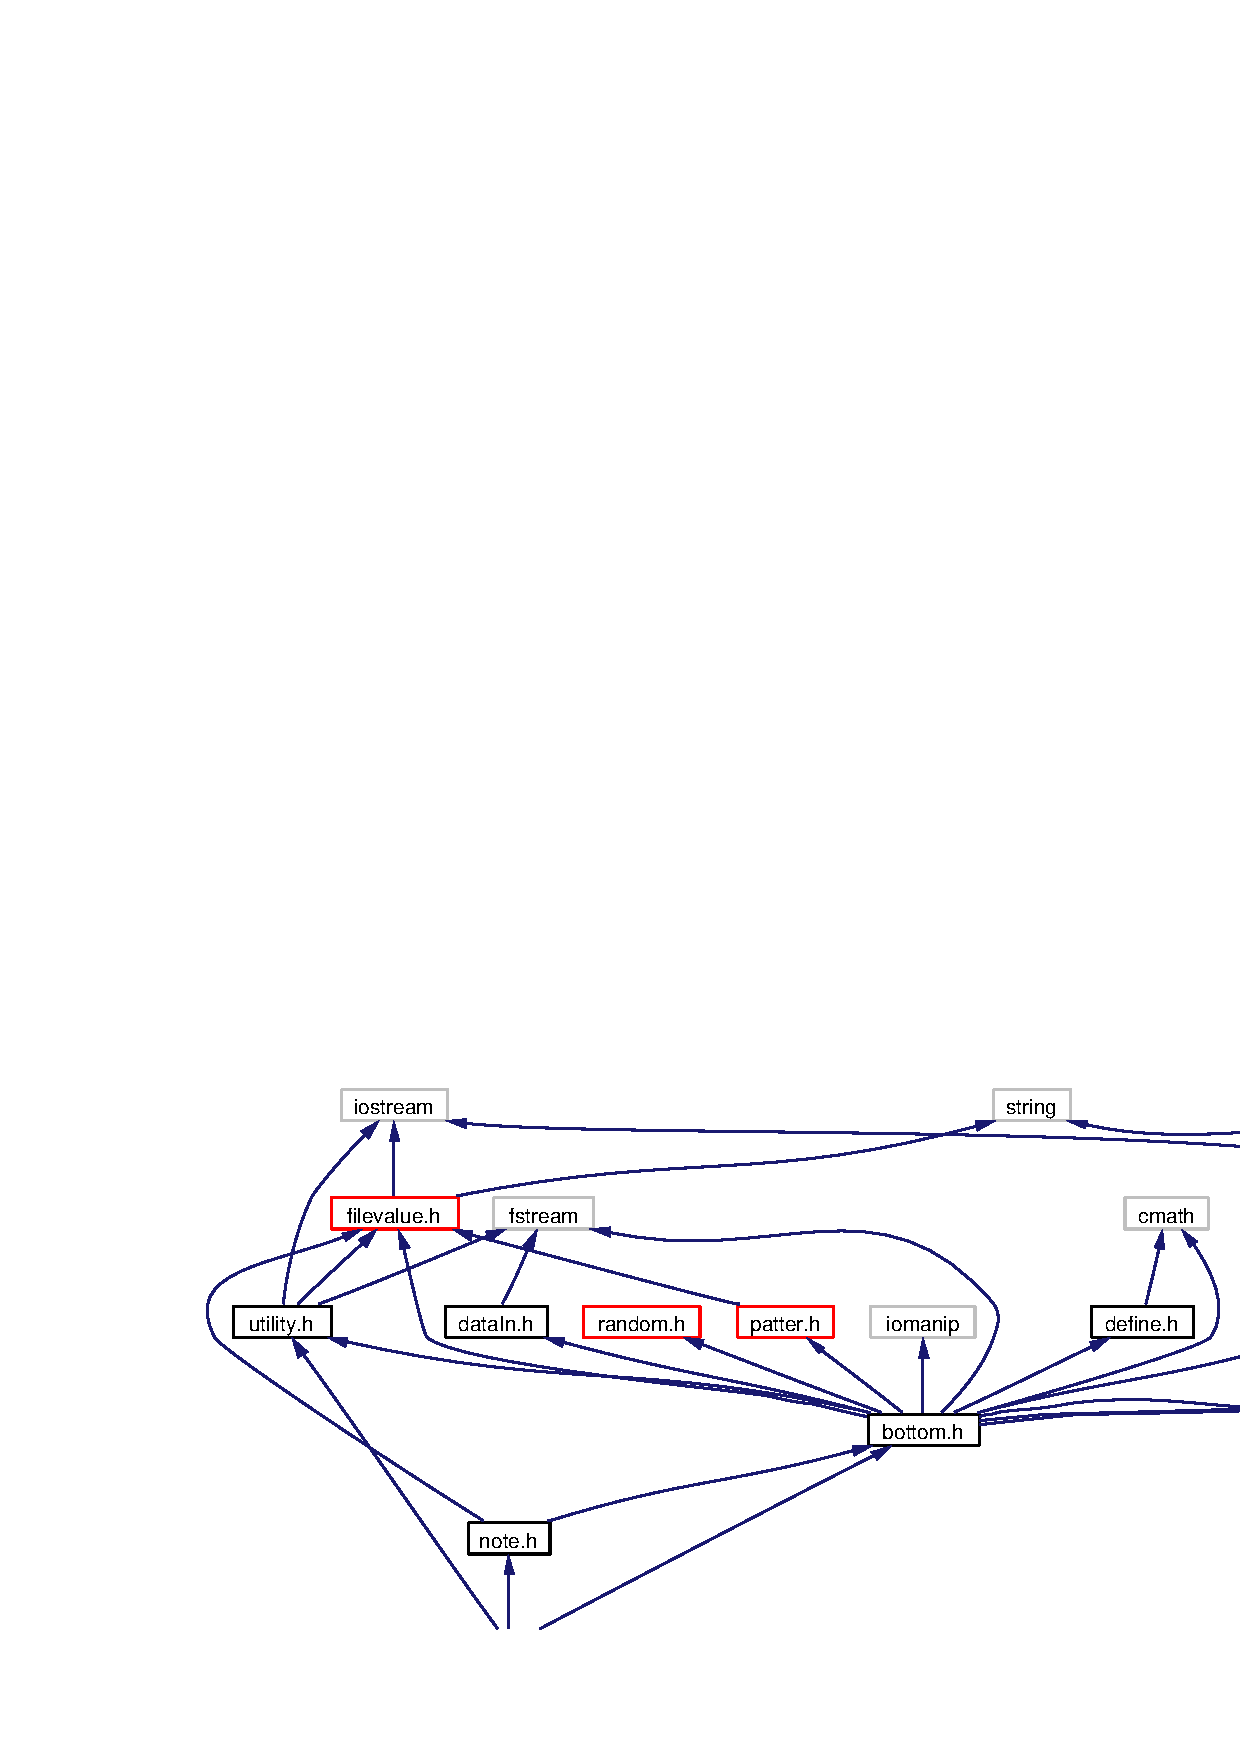
\includegraphics[width=393pt]{bottom_8cpp__incl}
\end{center}
\end{figure}
\subsection*{Namespaces}
\begin{CompactItemize}
\item 
namespace {\bf std}
\end{CompactItemize}
\subsection*{Variables}
\begin{CompactItemize}
\item 
ofstream $\ast$ {\bf output\-File}
\item 
Envelope\-Library {\bf envlib}
\item 
int {\bf bottom\-ID}
\item 
int {\bf note\-ID}
\item 
Score {\bf score}
\end{CompactItemize}


\subsection{Variable Documentation}
\index{bottom.cpp@{bottom.cpp}!bottomID@{bottomID}}
\index{bottomID@{bottomID}!bottom.cpp@{bottom.cpp}}
\subsubsection{\setlength{\rightskip}{0pt plus 5cm}int {\bf bottom\-ID}}\label{bottom_8cpp_a2}




Definition at line 32 of file bottom.cpp.

Referenced by Bottom::Bottom(), High::High(), Low::Low(), and Bottom::Print().\index{bottom.cpp@{bottom.cpp}!envlib@{envlib}}
\index{envlib@{envlib}!bottom.cpp@{bottom.cpp}}
\subsubsection{\setlength{\rightskip}{0pt plus 5cm}Envelope\-Library {\bf envlib}}\label{bottom_8cpp_a1}




Definition at line 31 of file bottom.cpp.

Referenced by Envelope\-Builder(), env\-Value(), Bottom::Modifiers(), Test\-Library(), and Bottom::Three\-Step().\index{bottom.cpp@{bottom.cpp}!noteID@{noteID}}
\index{noteID@{noteID}!bottom.cpp@{bottom.cpp}}
\subsubsection{\setlength{\rightskip}{0pt plus 5cm}int {\bf note\-ID}}\label{bottom_8cpp_a3}




Definition at line 33 of file bottom.cpp.

Referenced by Note::Note(), and Note::Print().\index{bottom.cpp@{bottom.cpp}!outputFile@{outputFile}}
\index{outputFile@{outputFile}!bottom.cpp@{bottom.cpp}}
\subsubsection{\setlength{\rightskip}{0pt plus 5cm}ofstream$\ast$ {\bf output\-File}}\label{bottom_8cpp_a0}




Definition at line 30 of file bottom.cpp.

Referenced by main(), Top::Print(), Note::Print(), Low::Print(), High::Print(), Bottom::Print(), and Bottom::Print\-Sound().\index{bottom.cpp@{bottom.cpp}!score@{score}}
\index{score@{score}!bottom.cpp@{bottom.cpp}}
\subsubsection{\setlength{\rightskip}{0pt plus 5cm}Score {\bf score}}\label{bottom_8cpp_a4}




Definition at line 34 of file bottom.cpp.

Referenced by Bottom::build\-Sound(), Event::Build\-Sub\-Events(), and main().